%----------------------------------------------------------------------------------------
%	Debug options
%----------------------------------------------------------------------------------------
% chktex-file 2
% chktex-file 8
% chktex-file 11
% chktex-file 13
% chktex-file 18
% chktex-file 36
% chktex-file 39
% chktex-file 44
%----------------------------------------------------------------------------------------
\chapter{Literature Review}\label{cha:LiteratureReview}
% # Why does this section matter?
% # How does it reflect on investigating the gap in Scrum
% # Transition to the next section
% What literature offers about the gap (Problems -> Solutions)
The literature review forms an important part of this thesis as it provides a comprehensive understanding of the existing body of knowledge on the theory-practice gap of Scrum. This chapter aims to identify and critically review previous studies, theories, and strategies related to the research questions and objectives. The literature review will provide a foundation for the research by highlighting the gaps in the existing knowledge and identifying areas that need further investigation.

The purpose of this chapter is to:

\begin{itemize}
    \item Provide an overview of Scrum methodology
    \item Explain the theory-practice gap of Scrum
    \item Identify the key theories, strategies, and studies related to the research questions and objectives
    \item Evaluate the strengths and limitations of previous research on the theory-practice gap of Scrum
    \item Identify the gaps in the existing body of knowledge that need further investigation
\end{itemize}

The literature review will be organized into sections based on the key themes and concepts that emerged from the review of the literature. This will provide a structured overview of the existing body of knowledge and highlight the key findings of previous research on the theory-practice gap of Scrum.

\section{Overview of the Scrum framework}\label{sec:OverviewScrumMethodology}
Scrum is a widely adopted \gls{framework} for Software Development and project management. As a \gls{framework}, Scrum was once only the \gls{methodology} of a few organizations and over time became a \gls{framework}. In \citeA[p.~3]{Schwaber2020Tsg} own words: "Scrum is a lightweight \gls{framework} that helps people, teams and organizations generate value through adaptive solutions for complex problems." The Scrum \gls{framework} is designed to help teams achieve their goals through a series of iterations and continuous improvement.

This section provides an overview of the Scrum \gls{methodology} by describing the origins, roles, events and artifacts that are part of Scrum and how they contribute to the success of the project.

% origins of Scrum
While originally invented by \citeA{Takeuchi1986TNN}, Scrum was first implemented as a \gls{framework} at the Easel Corporation and then first publicly presented in 1995 by Ken Schwaber and Jeff Sutherland at the Object-Oriented Programming, Systems, Languages and Applications (OOPSLA) Conference '95 in Austin, Texas. The name for the \gls{framework} stems from rugby, where it describes a formation of players. Today Scrum implies teamwork and collaboration as well as coordination. The first publication of the Scrum Guide was in the year 2010 as an effort to clarify what Scrum is and what it is not. The Scrum Guide refined on several occasions since~\cite{Kneafsey2015ASH}.

% what Scrum is now
The official Scrum Guide only serves the barebone explanation to incorporate Scrum in theory. It utilizes its abstractness to be more versatile. Rather than being a fixed process, accompanied by extensive documentation, it provides a set of \glspl{guideline} for the implemented interactions and relationships between roles.
Although trying to be abstract and versatile, the Scrum Guide also warns about changing the core design of Scrum by leaving out elements or ignoring the set rules of Scrum. By doing so a company does risk rendering the process useless or potentially even doing damage. An iterative and incremental approach in Scrum is used to optimize predictability and enhance the control of risk~\cite{Schwaber2020Tsg}.

% roles of Scrum
For Scrum to work, groups of people with all needed skills and expertise are needed to do or share the work between them. Responsible for all product-related activities from stakeholder collaboration, verification, maintenance, operation, experimentation, research and development, and anything else that might be required is the Scrum Team composed of Developers, a Scrum Master and a Product Owner~\cite[p.~5]{Schwaber2020Tsg}. Their definitions and responsibilities are as follows:

\begin{description}[style=nextline]
    \item[Developers]
    The Scrum Guide defines "\glspl{developer}" as encompassing all individuals involved in the development process, including architects and designers~\cite[p.~1]{Schwaber2020Tsg}. The Scrum team composition can be adjusted as required to meet the objectives of each sprint~\cite[p.~203]{Rubin2012ESA}. The Scrum approach prioritizes collaboration and cross-functional teams, giving the Scrum team the knowledge and expertise necessary to build the product increment, thereby reducing the risk of information loss compared to a \gls{plan-driven} approach. The diversity of skills and expertise among Scrum team members allows for the collective utilization of knowledge, leading to the creation of a thoughtful and valuable product.
    \item[Product Owner]
    The role of the \ac{po} is to optimize the value of the product and carry out various duties, including defining the product goal, establishing the product backlog with priorities, and responding to inquiries~\cite[pp.~5--6]{Schwaber2020Tsg}. The ideal \ac{po} should be the sole authoritative source with knowledge of the domain and comprehension of the needs of \glspl{client} and \glspl{customer}. To minimize confusion within the Scrum Team, it is recommended to appoint a single \ac{po} instead of a committee. However, in some organizations, an excessive workload may necessitate the division of responsibilities among multiple individuals, potentially reducing the capability of a single \ac{po} to effectively fulfill their responsibilities~\cite[p.~182]{Rubin2012ESA}.
    \item[Scrum Master]
    The role of the Scrum Master is crucial in facilitating the implementation of the Scrum \gls{framework}, not only in terms of theoretical understanding but also in terms of practical application. As specified in the Scrum Guide, the Scrum Master has the responsibility of promoting the \gls{adoption} of Scrum across the entire organization. The extent to which the Scrum Master can successfully integrate the Scrum \gls{framework} into the organization is dependent on the level of authority and influence they are granted by the organization~\cite[p.~6]{Schwaber2020Tsg}.
\end{description}

% events of Scrum
The Scrum \gls{framework} utilizes specific events during a sprint to raise transparency, inspection and adaption~\cite[p.~3]{Schwaber2020Tsg}. These events are as follows:

\begin{description}[style=nextline]
    \item[Sprint]
    The Sprint, as defined by the Scrum Guide, is a time-bound event that encompasses all other events in the \gls{framework}. During a Sprint, changes that would jeopardize the achievement of the Sprint Goal are not allowed. The Product Backlog may be continuously refined and its scope clarified and renegotiated with the \ac{po}. Sprints offer the advantage of synchronizing work with other teams, promoting collaboration and reducing the waste of time and effort on non-value-adding tasks. This protected \gls{framework} increases the reliability of the system towards stakeholders and enhances the ability of all parties to plan and coordinate effectively.~\cite[pp.~7--8]{Schwaber2020Tsg}
    \item[Sprint Planning]
    The Sprint Planning event involves the participation of all Scrum Team members to define a shared understanding of the work results to be delivered, referred to as the Sprint Goal. This event promotes clarity and reduces misunderstandings by defining the purpose, scope, and approach of the work to be executed in the upcoming Sprint. By planning and defining what should and should not be done during the Sprint, supported by the experts of the team, this event helps to minimize the impact of changing requirements and distractions from non-critical tasks, resulting in more efficient use of time and resources.~\cite[p.~8]{Schwaber2020Tsg}
    \item[Daily Scrum]
    The Daily Scrum is a collaborative event aimed at inspecting the progress towards the Sprint Goal and adapting the Sprint Backlog. This process facilitates mutual assistance and makes team barriers visible, reducing the need for multiple meetings and allowing for longer periods of focused work. As a result, the quality of the product is improved. The Daily Scrum is not designed for management control, but rather for team collaboration and progress monitoring.~\cite[p.~9]{Schwaber2020Tsg}
    \item[Sprint Review]  
    The Sprint Review serves as a platform for the Scrum Team to demonstrate and assess their progress toward the Product Goal with stakeholders. Through this interactive session, the team can identify dependencies and make necessary adjustments to the Product Backlog. The Sprint Review should not be considered a presentation, but rather a collaborative working session.~\cite[p.~9]{Schwaber2020Tsg}
    \item[Sprint Retrospective] 
    During a Sprint Retrospective, the Scrum Team engages in a collaborative examination of their process and performance with the aim of identifying and implementing improvements. Moderated by the Scrum Master, the team focuses on the interactions, processes, tools, and individuals involved, rather than the specific work results. The outcome of the Sprint Retrospective is an increased level of awareness, effectiveness, and reduced potential for conflict and frustration within the team.~\cite[p.~10]{Schwaber2020Tsg}
\end{description}

% artifacts of Scrum
The Scrum \gls{framework} defines three primary artifacts in order to manage the workload:

\begin{description}[style=nextline]
    \item[Product Backlog]
    The Product Backlog is a prioritized list of items that describe the functional and non-functional requirements of the product, including features, enhancements, and bug fixes. The list is continually refined and updated based on the Product Goal, and is never considered to be a comprehensive or final representation of the product's requirements. The prioritization of the items in the Product Backlog is determined by the \ac{po} and represents their understanding of the relative importance of the items in achieving the Product Goal.~\cite[pp.~10--11]{Schwaber2020Tsg}
    \item[Sprint Backlog]
    The Sprint Backlog is a dynamic list of items compiled by the development team that outlines the work they have committed to completing during a specific Sprint. It is subject to change and \gls{adaptation} as the Sprint progresses and is maintained exclusively by the development team. The amount of detail it holds has to be sufficient to inspect the progress towards the Sprint Goal~\cite[p.~11]{Schwaber2020Tsg}
    \item[Increment]
    The Increment is a critical component, serving as a tangible representation of progress towards the Product Goal. It is created through the addition of work items that have been verified to meet the \gls{dod}, ensuring that each Increment is usable and integrates seamlessly with prior Increments. The creation of multiple Increments within a Sprint is supported by empiricism, and their sum is presented at the Sprint Review. It is important to note that work cannot be considered part of an Increment unless it has met the established \gls{dod}.~\cite[pp.~11--12]{Schwaber2020Tsg}
\end{description}

% Agile Software Development
Although never stated in the Scrum Guide directly, the \gls{methodology} of Scrum overlaps with the one of \acf{asd} and could be viewed as a practical application of \ac{asd}. That said, Scrum could be implemented without the integration of the \ac{asd} \gls{mindset}~\cite[p.~56]{Moreira2013FoA}, although the organization would probably not benefit as much from Scrum~(\citeNP[p.~123]{Moreira2013AtA};~\citeNP[pp.~7--9]{Bannink2014Cit}). The goal of \ac{asd} is to deliver working software to \glspl{client}, while still considering sustainability and clear documentation. Despite the lack of explicit planning and risk management in the \ac{agile-manifesto}, the approach is not inherently riskier~\cite[p.~3]{battoia2019innovation}. Instead, it prioritizes collaboration with \glspl{client} and values their role in the project's success. The use of incremental payments and sprints helps mitigate the risk of scope creep, while also allowing for a more flexible and adaptive design process in response to changes~\cite{Beck2001MfA}.

\quotethis{Agile:\newline
Work small, Talk to each other, Make people’s lives better\newline
That's it. All that other junk is a distraction.}{\citeNP{AllenHolub2022AW}}

\newpage
\takeaways{
    In this section, the fundamental \glspl{principle} of the Scrum \gls{methodology} and its key components were presented as a foundation for the exploration of the theory-practice gap of Scrum. Scrum is a \gls{framework} that originated from a functional \gls{methodology}, meaning its \glspl{method} have been tested and applied within teams. However, the efficacy of the \gls{methodology} is contingent on its compatibility with a particular team. Although Scrum can be utilized without the \ac{asd} mindset, this is unlikely to lead to optimal results as Scrum is rooted in the \gls{agile} \gls{methodology}. Hence, both the \gls{ideology} of \ac{asd} and the \gls{methodology} of Scrum are necessary for Scrum to function effectively. It is important to note that adopting Scrum does not automatically translate to being \gls{agile}. Additionally, the \gls{agile} approach is not inherently riskier than traditional waterfall processes as the \gls{client} retains control throughout the project and can decide to discontinue the project at any time while still retaining a usable product concept.
}

\section{Explanation of the theory-practice gap of Scrum}\label{sec:ExplanationGapScrum}
% Summary and goals for the section
% Why it is important for the research question
% What this section will add to the thesis
This section aims to clarify the concept of the theory-practice gap of Scrum by providing clear definitions of the terms "theory" and "practice". The distinction between "theory" and "ideology" will also be discussed. A comprehensive overview of the general theory-practice gap will be presented, including its common dimensions and forms. Lastly, a characterization of the specific theory-practice gap within the context of Scrum will be provided. The resulting frame will be the foundation for the contribution of this thesis.

% What is "theory"
According to the theorization by \citeA{Wacker1998Ado}, theory serves as an abstraction of a portion of reality, aimed at providing explanatory insights into the pragmatic world. \citeA{Carr1980TGb} further elaborates that theory and practice are not inherently linked, but rather theory influences practice through a critical and rational analysis that assesses and justifies the practices, leading to the evolution and \gls{transformation} of the way in which practice is understood and experienced. This process can also be observed in the development and refinement of the Scrum Guide. For a more in-depth definition of theory, the research done by \citeA{Moustafa2014DoT} is recommended.

% What is the difference between "theory" and "ideology"
The difference between theory and \gls{ideology} can be best understood by examining the \gls{mindset} of individuals. A \gls{mindset} is a cognitive orientation, characterized by patterns of thoughts, attitudes and beliefs towards reality and the self. It is often established as a habit~\cite{Dictionary2022ME, 2018IvM}. When individuals share a common set of beliefs, they form a collective ideology, which encompasses a doctrine, philosophy, or set of values informed by underlying \glspl{principle}~\cite{Dictionary2022IE, 2018IvM}. In contrast, theory aims to provide explanations, descriptions, and predictions of interactions and behaviors~(\citeNP[pp.~361--363]{Wacker1998Ado};~\citeNP{Dictionary2022TE}). For a more in-depth definition of ideology, the research done by \citeA{Moramollu2016Ial} is recommended.

The distinctiveness of theory and \gls{ideology} is depicted in Figure~\ref{fig:theory-ideology}.

\newpage
\begin{figure}[!h]
	\begin{center}
        \makebox[\textwidth]{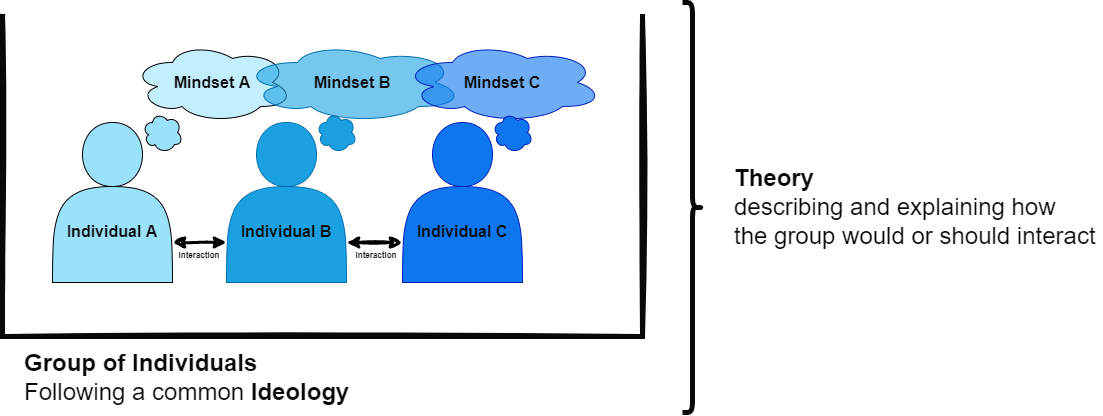
\includegraphics[width=\textwidth]{./assets/images/ideology-mindset-theory.png}}
        \caption{Visualization of the interaction between ideology and theory}\label{fig:theory-ideology}
    \end{center}
\end{figure}

% What is "practice"
\citeA[pp.~3--5]{Wenger1998Cop} posit that there exist various types of groups for practices, each of which can be at a different stage of development, ranging from the formation of a community to its eventual dissolution. The choice of Scrum as a \gls{framework} and \ac{asd} as a \gls{mindset} can vary, with the success of these choices being contingent on the nature of the group. According to \citeA[p.~5]{Wenger1998Cop}, communities can have five different relationships with organizations, with those that are unrecognized or bootlegged not contributing to organizational \gls{transformation} due to a lack of maturity and size. On the other hand, a community that is legitimized, seen as strategic, or transformative can have a significant impact and receive support from the organization it aims to transform or improve.

% What is a gap in theory and practice
The theory-practice gap is a long-debated concept among scientifically oriented philosophers, who question the practical implications of theories~\cite[p.~61]{Carr1980TGb}. According to \citeA[p.~2]{Greenway2019Wia}, while there are various unclear definitions of a theory-practice gap, research into it is often aimed at improving communication between the two. \citeA[p.~60; p.~65]{Carr1980TGb} cites the difficult jargon of theories as a possible reason for the gap, as well as differences in language and evaluation criteria between theorists and practitioners. \citeA[p.~63]{Carr1980TGb} suggests that the gap often arises from methodological problems and can be solved by changing the \gls{methodology} through new insights from practitioners. He also writes that the theory-practice gap can only be closed by involving practitioners in the solution development process, rather than relying solely on theorization and \glspl{guideline}. An integrated or problem-based approach is unlikely to lead to satisfactory results. The active participation of practitioners is essential in enhancing the theoretical field.~\cite[p.~67]{Carr1980TGb}

% What Attributes does it take on
The theory-practice gap can therefore be characterized in three dimensions: language, evolution, and \gls{methodology}. The language dimension refers to the cause of the gap due to specialized jargon in theory or lack of understanding in practice. The \gls{methodology} dimension highlights the causes of the gap between theory and practice through the theory not being derived from the actual practices of practitioners, not being suited for the activities faced by practitioners, or evaluating success differently. The evolution dimension illustrates the cause of the gap due to the theory lagging behind advancements in practice.

The dimensions and attributes of a general theory-practice gap derived from the previous paragraphs are visualized in Figure~\ref{fig:gap-attributes}

\begin{figure}[!ht]
	\begin{center}
        \makebox[\textwidth]{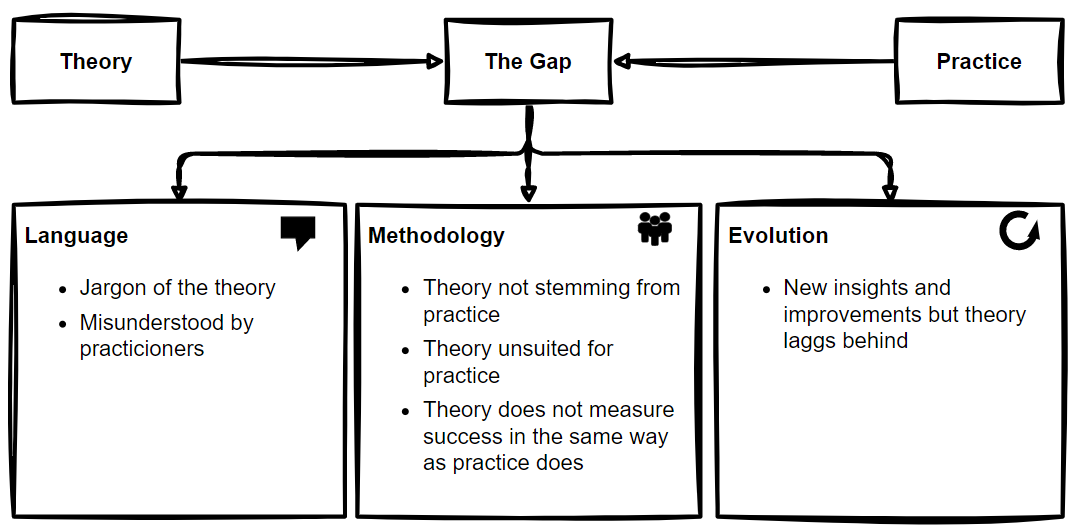
\includegraphics[width=\textwidth]{./assets/images/attributes-dimensions-gap.png}}
        \caption{A general theory-practice gap and its attributes and dimensions derived from Carr's description}\label{fig:gap-attributes}
    \end{center}
\end{figure}

% What Attributes does the gap of Scrum take on
Utilizing the model for a general gap in theory and practice, the gap in the context of Scrum can be attributed as follows:

The first dimension, Language, is characterized by specialized jargon in the theory of Scrum, as well as misunderstandings and misconceptions about Scrum's \glspl{method}. The abstractness of the Scrum Guide, as an example, could therefore lead to discussions about who is meant by the role \glspl{developer}, since the common association with this role are programmers. This can lead to questions about the effectiveness of Scrum since a misunderstanding regarding the role of the \gls{developer} could lead to arguments such as Scrum lacking upfront design. The lack of clear verbalization of risk management in the Scrum Guide is another example of a possibility of miscommunication, since some may argue that missing risk management leads to riskier projects. 

The second dimension, \Gls{methodology}, is the largest of the gap and is characterized by difficulties in transforming or merging existing \glspl{methodology}, roles or control structures, budgeting training, and scaling self-management and self-organization to larger teams. A common problem with the \gls{transition} from a \gls{plan-driven} process to Scrum can be the \gls{transformation} of management roles since in Scrum, managers no longer micromanage but instead become servant leaders.

The third dimension, Evolution, is characterized by the challenge of scaling Scrum beyond the initial idea of small \gls{self-managing} teams and single projects and finding a \gls{framework} that enables teams of teams to deal with multiple projects at the same time. An example of this could be the divergence of the \glspl{framework} for scaling Scrum. Some stay true to the \gls{agile} \gls{ideology} while some reintroduce command-and-control structures.

These examples illustrate how the theory-practice gap can lead to Scrum being less effective than it was intended to be and highlight the importance of continuously revisiting and adjusting the way Scrum is being implemented to ensure that it aligns with the underlying \glspl{principle} and values of the \gls{framework}.\newline
The derived model for Scrum's gap of theory and practice is visualized by Figure~\ref{fig:gap-attributes-scrum}.

\begin{figure}[!ht]
	\begin{center}
        \makebox[\textwidth]{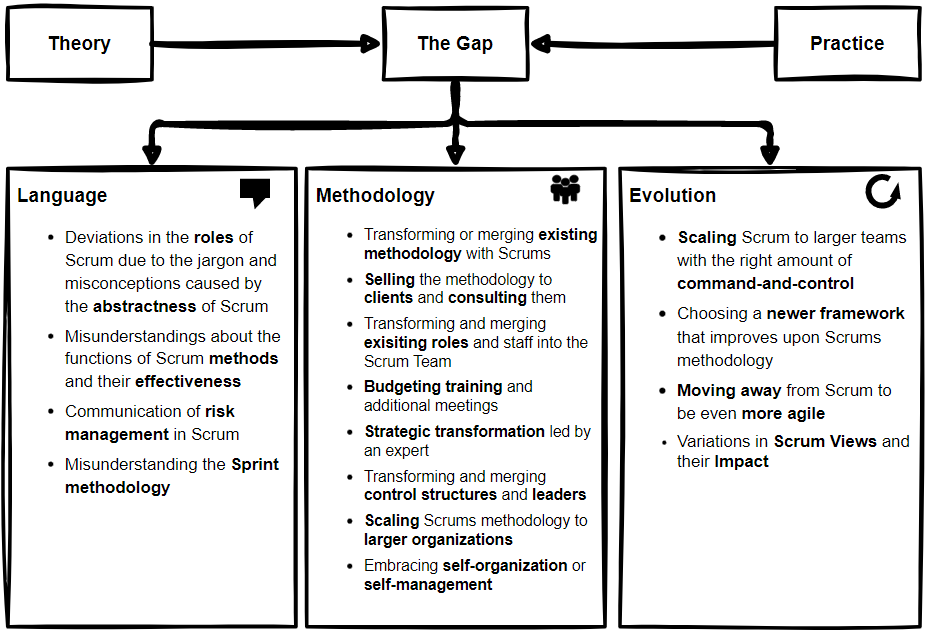
\includegraphics[width=\textwidth]{./assets/images/attributes-dimensions-gap-scrum.png}}
        \caption{The theory-practice gap of Scrum and its attributes and dimensions}\label{fig:gap-attributes-scrum}
    \end{center}
\end{figure}

\takeaways{
    The gap between theory and practice in Scrum can be defined as the difference between the concepts and models presented in Scrum literature and the actual implementation and application of these concepts in real-world scenarios. The theory-practice gap can be divided into three dimensions: language, \gls{methodology}, and evolution. Previous studies have shown that effective communication and bridging the gap can be achieved through the development of practical solutions by practitioners, rather than relying solely on theory and \glspl{guideline}. The Scrum gap has several attributes including deviations in roles due to misunderstandings in the abstract Scrum Guide, perceived higher risk compared to traditional development \glspl{method}, the ineffective merging of traditional \glspl{methodology} with the Scrum framework, lack of expert-guided \gls{transformation} planning, difficulties in embracing self-organization and self-management, and scaling challenges due to the addition of command-and-control structures and the selection of inappropriate \glspl{framework}.
}

\newpage

\section{Previous studies on the theory-practice gap of Scrum}\label{sec:PreviousStudies}
% # Identify the key theories, strategies, and studies related to the research questions and objectives
% # Evaluate the strengths and limitations of previous research on the theory-practice gap of Scrum
% Purpose of the section
% Significance of examining previous studies
Previous studies on the theory-practice gap of Scrum have explored the reasons for this disparity, focusing on various factors such as misunderstandings, lack of training, and difficulty in scaling Scrum to larger organizations. This section aims to provide a comprehensive review of these previous studies, highlighting key findings and offering insights into the current state of knowledge on the theory-practice gap of Scrum. By doing so, this section will lay the foundation for a deeper understanding of the challenges and opportunities associated with bridging the gap between Scrum theory and practice.

% Overview of previous studies
% Theoretical foundations of previous studies
\subsection*{Historical evolution of Scrum}\label{subsec:historyOfScrum}
The historical evolution of Scrum can be traced back to its origins in the mid-1990s when Ken Schwaber and Jeff Sutherland developed the Scrum \gls{framework}. They have tested the Scrum \gls{methodology} in some organizations and found it to be valuable.

With the first iterations of the Scrum Guide clarifying what Scrum is and introducing flexibility to the \gls{framework} in order to be widely adoptable, it visualizes the increasing interest in developing in a more \gls{agile} manner. But with the broader interest may have come some misconceptions about the values and \gls{methodology}, which led to the introduction of the key values and an emphasis of transparency. The events of Scrum, for example, the Daily Scrum, had been specified and artifacts and their handling described.~\cite[Revision 2010--2013]{Schwaber2020SGR}

Scrum's success had led to the development of \glspl{framework} encompassing Scrum's \gls{methodology} or parts of it and being targeted at more specific demographics, for example, scaling \glspl{framework} such as the \ac{safe} and \ac{less}. This may have led to the Scrum Guide clarifying that Scrum in essence is still made for smaller teams. They enforced the meaning of servant-leaders and the role of the Scrum Master accordingly. In addition, they emphasized the benefits of working in small teams and explained that they could be kept by having networks of small teams and avoiding introducing command-and-control structures.~\cite[Revision 2013--2017]{Schwaber2020SGR}

In the latest revisions, Scrum has been reduced to being a minimally sufficient framework, with an emphasis on a small team working together, the Scrum Team. It was described that way because the authors of the Scrum Guide wanted to clarify, that the Scrum Team does collaborate closely and does not have frequent handovers like the former \gls{plan-driven} approaches had between departments. This revision also clarified the artifacts to make them easier understandable. In order to be understood by a wider audience, the Scrum Guide has been simplified in the language by eliminating redundant, complex statements and removing any remaining reference to IT. This is probably due to Scrum encompassing a wider range of domains and industries, including product development, healthcare, and education.~\cite[Revision 2017--2020]{Schwaber2020SGR}

Overall, the historical evolution of Scrum reflects the growing popularity and acceptance of the Scrum \gls{framework}, as well as the ongoing efforts to refine and improve its practices and outcomes.

% Explanation of relevant theories related to the theory-practice gap
% Summary of key findings from previous studies
% Comparison of previous studies in terms of research methodologies, sample populations, and outcomes
% Overview of how previous studies have applied these theories to Scrum
\subsection*{Summary of key findings from previous studies}
In the field of Scrum, numerous studies have been conducted over the years to uncover its various aspects, benefits, and limitations. This body of research has helped to establish Scrum as a popular \gls{framework} for \ac{asd} and provided insight into its implementation and use in organizations. This section will provide a summary of the key findings from previous studies that have been conducted on Scrum. The objective of this summary is to provide a comprehensive understanding of the research that has been done in this field and highlight the key insights and trends that have emerged from these studies. These key findings will be sorted by their associated dimension and attribute derived from the Figure~\ref{fig:gap-attributes-scrum}.

\subsubsection*{Deviations in the roles of Scrum}\label{subsubsec:DeviationOfRoles}
The integration of Scrum as a \gls{methodology} can be problematic for some organizations, as indicated by \citeA[p.~1]{Diebold2015Wdp} who found that only one-fourth of organizations using Scrum followed the \glspl{guideline} set forth in the Scrum Guide. Misunderstandings of roles within the team can lead to frustration, as stated by \citeA[p.~29]{Koning2019AT}. Even though the Scrum Guide defines anyone who feels included as a \gls{developer}, additional roles such as \ac{ux} designer get added to the Team. Organizations often turn to external experts to aid in the integration of Scrum~(\citeNP[p.~5]{Bannink2014Cit};~\citeNP[p.~2]{Sidky2007ADA}). This raises questions about the effectiveness of certified Scrum Masters in actually executing the integration and training process. On the other hand, organizations utilizing scaling \glspl{framework} for Scrum frequently utilize these external experts~(\citeNP[p.~1]{Paasivaara2016SSi};~\citeNP[p.~6999]{Moe2019Tai}). Further research is needed to confirm these conclusions, as the literature provides no clear answer.

\subsubsection*{Misunderstandings about the functions of Scrum methods and their effectiveness}\label{subsubsec:MisunderstandingsOfScrum}
\citeA[p.~3]{Reddy2021HMU} argue that Scrum does not put enough emphasis on conception, leading to potential refactoring. \citeA[p.~56]{Moreira2013FoA} acknowledges that Scrum can be integrated into a \gls{plan-driven} process. Scrum and \ac{asd} are different but often used together, leading to misinterpretation due to lack of understanding. Scrum provides \glspl{method} while \ac{asd} provides \gls{mindset} and values, but Scrum without \ac{asd} lacks the essence of its \gls{methodology}. New organizations may find the abstractness of Scrum definitions misleading. With valuable increments each Sprint, Scrum delivers more frequently than \gls{plan-driven} approaches~\cite[p.~34]{Rubin2012ESA}.

\subsubsection*{Communication of risk management in Scrum}\label{subsubsec:RiskManagementInScrum}
Risk management in \ac{asd} reduces the risk of developing a non-viable or non-desirable product through collaboration with the \gls{client} and planning each sprint~\cite[p.~18]{battoia2019innovation}. The \gls{client} benefits from frequent releases~\cite[p.~4]{RachevaCpi} and direct communication with the team, leading to faster feedback and reduced miscommunication~\cite[p.~193]{Cho2008IAC}. The \gls{transition} to an \gls{agile} approach requires the \gls{client} to understand their impact on prioritizing the backlog and the benefits of using use-cases and removing feedback loops~(\citeNP[p.~153]{mancl2019xp};~\citeNP[p.~36]{Boehm2005Mct}). 

This results in higher-quality products, increased \gls{adaptation} to changes, and improved \gls{customer} satisfaction~\cite[p.~99]{Abrahmson2002ASD}. Detecting problems early on and short communication channels between the team and \gls{client} lead to more efficient resolution of issues.

\subsubsection{Misunderstanding the sprint methodology}\label{subsubsec:UnderstandingSprints}
The Sprint \gls{methodology} is a fixed-length event of one month or less designed to achieve consistency in product development~\cite[p.~7]{Schwaber2020Tsg}. It is commonly utilized for achieving a specific goal, such as the Product Goal, but it is not limited to software development. Instead, it enables cross-functional teams to build functional increments that can be shared across teams. This approach offers several benefits.

The full application of the Sprint \gls{methodology} involves a \gls{client} contracting an organization to develop their product. A Concept Sprint can be used to test the waters and develop a product vision under the guidance of the \gls{client}. If the \gls{client} is satisfied with the work, they can continue with the development by paying for each subsequent sprint, which will deliver a functional and valuable increment prioritized by value. If the product reaches a fully functional state, the Scrum Team can use Enhancement Sprints to incorporate product backlog items that were not deemed important earlier~\cite[p.~2]{Sutherland2005Fos}.

The Sprint \gls{methodology} can also be applied within an organization through Integration Retrospectives and Enhancement Sprints to improve processes. This would enable organizations to reflect on their progress towards being more adaptive and \gls{agile} and how they can optimize their way of working, effectively treating their processes as a product they continuously develop and improve~\cite[pp.~395--396]{Rubin2012ESA}.

\subsubsection*{Transforming or merging exsisting methodology with Scrums}\label{subsubsec:TransformingTheMethodology}
Scrum is a \gls{methodology} that can be used by development departments but it can only reach its full potential if the entire organization embraces it~(\citeNP[p.~233]{Rubin2012ESA};~\citeNP[p.~15]{Maximini2018ISi}). According to the \citeA{20211AS}, the main challenge to adopting and expanding \gls{agile} practices is inconsistent processes and practices across teams.

\subsubsection*{Transforming and merging existing roles and staff into the Scrum Team}\label{subsubsec:TransformingRoles}
\citeA[p.~214]{Rubin2012ESA} argues that to fully realize the benefits of Scrum, the entire organization should embrace it and the \ac{asd} \gls{ideology}. For example, the role of \ac{ui} designer should be part of the Scrum Team to reduce communication time and allow for easier change management, but would be also described as a \gls{developer}~\cite[p.~214]{Rubin2012ESA}. The role of the Requirement Engineer is absorbed into the role of the \ac{po}, who takes on responsibility for refining requirements~(\citeNP[pp.~5--6]{VanLamsweerde2000Rei};~\citeNP[p.~127]{Maximini2018ISi}). \Acp{pm} are no longer needed~\cite[p.~239]{Rubin2012ESA} and the \ac{po} takes over their responsibilities, though some organizations still keep \acp{pm} or use them for delegation~(\citeNP[p.~239]{Rubin2012ESA};~\citeNP[p.~73]{Maximini2018ISi}).

The role of the salesperson should not be added to the Scrum Team but rather the \ac{po}'s responsibilities should be expanded to include \gls{client} communication and negotiation~\cite[pp.~34--35]{Boehm2005Mct}. Management plays a crucial role in the \gls{transition} to Scrum~\cite[p.~16]{Moreira2013AtA} and needs to be involved and adopt new responsibilities, but if they lack expertise in \gls{agile}, a coach or expert should be consulted~\cite[p.~77]{Moreira2013AtA}. Management should have trust in the development team and empower employees to make decisions without upper management involvement~\cite[p.~34]{Moreira2013AtA}.

\subsubsection*{Transforming and merging control structures and leaders}\label{subsubsec:TransformingManagement}
In the field of software development, transforming existing control structures is seen as important for the success of \gls{agile} \glspl{methodology} such as Scrum. \citeA[p.~6]{Jilani2020ItG} recommend a gentle approach to reducing command and control structures, as well as changing culture and leadership in the organization (\citeNP[p.~4]{Barroca2019Ata};~\citeNP[p.~15]{Rubin2012ESA}). In Scrum, the \ac{po} provides product leadership~\cite[p.~15]{Rubin2012ESA} while the Scrum Master provides process leadership~\cite[p.~16]{Rubin2012ESA}, and other leadership roles are more focused on developing skills among team members~\cite[p.~56]{Alami2022HSa}. Leaders need to be properly skilled and distributed across different products, and the ideal situation is where everyone leads themselves~\cite[p.~39]{Moreira2013AtA}. The \ac{po} is the single authority for deciding what the Scrum Team should work on, while the Scrum Master removes obstacles. The Scrum Master's leadership style is described as \gls{agile}, accountability, or servant leadership, while the \ac{po}'s is described as transparency leadership~\cite[p.~56]{Alami2022HSa}. In contrast, traditional approaches to management and leadership follow a transactional leadership style, which is focused on directing and assigning work~(\citeNP[p.~124]{Moreira2013AtA};~\citeNP[p.~101]{Uwadi2022RoM}). Psychological and technical leadership are also important for creating a safe work climate and providing support for the team ~(\citeNP[p.~56]{Alami2022HSa};~\citeNP[p.~64]{Abrahmson2002ASD}). To be successful, the organization must move away from a centralized decision-making model~\cite[p.~152]{mancl2019xp} and towards a flat team model where everyone is a leader~\cite[p.~129]{Moreira2013AtA}. Therefore, middle management must change roles, becoming servant leaders who support the Scrum Team and manage resources, rather than assigning work~\cite[p.~125]{Moreira2013AtA}.

\subsubsection*{Selling the methodology to clients and consult them}\label{subsubsec:SellingScrum}
The client's involvement is crucial for the success of the project and collaboration with them is more valuable than contract negotiation. 60\% of project risks can be linked to the client, and involving them directly and training them can help mitigate these risks~\cite[p.~5]{Coyle2009Acs}. The concept of incremental payment limits the \gls{scope-creep} and helps the product become more refined~\cite{Beck2001MfA}. The \ac{po} holds all the necessary knowledge about the product and should be a domain expert if the product is outsourced~\cite[p.~180]{Rubin2012ESA}. For prioritization of the backlog items, the discussion between the \ac{po} and development team is a necessity~\cite[p.~2]{Rajasekaran2015IiS}. Contracting should not be seen as a fixed-price contract but rather as leasing the Scrum Master and development team~\cite[p.~180]{Rubin2012ESA}. \Glspl{client} only pay for sprints with specific goals that are prioritized by the \ac{po}, and each sprint must be a functional product. The \gls{client} can end the development at any time and keep the functional product developed until then. This results in the right product being built and higher \gls{client} satisfaction.

\subsubsection*{Budgeting training and additional meetings}\label{subsubsec:BudgetingTrainging}
Investing in training is recommended to align staff in a common \gls{mindset} and improve product selling, according to \citeA[p.~72]{Maximini2018ISi}. The \gls{agile} approach to Software Development focuses on building the best product possible, rather than blindly following trends. The team should consider the client's needs before investing in new technologies~\cite[p.~43]{Maximini2018ISi}. A successful \gls{transition} to Scrum requires planning and upper management support~(\citeNP[p.~183]{Jilani2020ItG};~\citeNP[pp.~37--38]{Boehm2005Mct}). Resistance to change and conflicts can be solved with training and the involvement of an \gls{agile} Coach~\cite[p.~21]{Naseem2009Saa}. Aligning \glspl{mindset}, explaining roles and \glspl{method}, and highlighting benefits are advised to prevent upper management from falling back to traditional command-and-control leadership~\cite{Moreira2013AtA}.

\quotethis{Educating a team slows you down for a week or two. Not educating the team slows you down forever. Time spent in learning is never wasted.}{\citeNP{AllenHol71}}

\subsubsection*{Strategic transformation led by an expert}\label{subsubsec:StrategicTransformation}
The use of the Scrum \gls{framework} may not be suitable for every organization and it is important for each organization to carefully consider whether the \gls{ideology} of \ac{asd} fits their needs. It is not recommended to blindly follow a trend without evaluating its potential benefits and drawbacks~\cite[p.~152]{Meyer2014ABM}. The best way to achieve alignment within an organization is to involve employees in decision-making and find a common ground that works for everyone. Collaboratively made decisions and \gls{commitment} to them form the basis for alignment~\cite[p.~6997]{Moe2019Tai}.

To keep employees aligned, it is important to prioritize retrospective and alignment meetings and treat them with respect~\cite[p.~28]{Uludag2019Ita}. Unfortunately, only a small percentage of employees feel that their organization supports the \gls{agile} culture~\cite[p.~27]{Koning2019AT}. Culture has the biggest impact on \glspl{transformation}, as structures, processes, and technologies cannot adapt without a change in the way people work and collaborate~\cite[pp.~31--32]{Thorgren2019Tro}. A collaborative culture also enables employees to improve their learning and health through shared knowledge and responsibility~\cite[p.~32]{Thorgren2019Tro}.

A crucial aspect of a collaborative culture is psychological safety, which includes inclusiveness, perceived trust in collective responsibility, and openness in communication. If psychological safety is not present, employees may revert back to fear-based norms and not feel comfortable presenting their ideas or asking for help~\cite[p.~5]{Alami2022HSa}. To foster a collaborative culture, everyone from the \gls{developer} to the manager must work together and commit to cultural change. If there is a struggle in achieving this, it may be necessary to bring in an experienced coach to help with the \gls{transition}~\cite[p.~237]{Moreira2013AtA}. \citeA[p.~37]{Thorgren2019Tro} recommend exploring different cultures that could be involved in the \gls{transition} and prioritize psychological safety in the process. This exploration can provide valuable insights and help with cross-cultural implementations, but it is important to consider potential cultural clashes and the impact they may have on employee \glspl{mindset}.

\subsubsection*{Scaling Scrums methodology to larger organizations}\label{subsubsec:ScalingScrum}
When transitioning to more teams it is important to keep the teams running. The Dreyfus Squared Model provides guidance on creating effective pairs in teams to achieve innovative solutions~\cite{North2022PoE}. Alignment and planning meetings are important for teams to work effectively on a product in parallel~\cite[p.~57]{guide13scrum}. The Scrum Guide recommends the Daily Stand Up and Sprint Planning meetings to help the team share a common vision for the product. Regular collaboration with other team members helps maintain motivation~\cite[p.~7]{Zikopi2019Acs}. A strong Team Lead such as the Scrum Master and the \ac{po} can help eliminate distractions~\cite[p.~21]{Naseem2009Saa}. Effective Teams balance accountability and the need for breaks to avoid overworking team members~\cite[p.~137]{Rubin2012ESA}.

\subsubsection*{Embracing self-organization or self-management}\label{subsubsec:EmbracingSelfManagement}
The concept of \gls{self-managing} and \gls{self-organizing} systems refers to systems that are able to adapt to changes without external control. These systems take inputs from the environment and generate control inputs based on their current and past inputs, thus allowing for \gls{adaptation}. While \gls{self-managing} systems generate their control inputs independently, \gls{self-organizing} systems interact with each other to provide the system's primary functionality and can even restructure the entire system when necessary~\cite[pp.~4--5]{Muehl2007Otd}.

According to \citeauthor{Schwaber2020SGR}, the definition of development teams in the Scrum Guide has changed from being \gls{self-organizing} to \gls{self-managing}, giving teams the authority to decide who, what, and when to work on the product. However, this shift in terminology may result in differing interpretations of the concept of self-management.

\Gls{self-managing} teams can lead to higher productivity as they work mostly autonomously, proactively manage tasks, and make decisions through a transparent hierarchy and collaboration of ideas and knowledge \cite[p.~56]{Muthusamy2005Smw}. The close collaboration results in higher \gls{commitment}, \gls{ownership}, and improved employee satisfaction~\cite[p.~142]{Rubin2012ESA}. By eliminating the loss of information between departments or silos of experience~(\citeNP[p.~119]{blunden2010clean};~\citeNP[p.~210]{Rubin2012ESA}), cross-functional \gls{self-managing} teams result in better-constructed products with a focus on quality and less waste~\cite[p.~142]{Rubin2012ESA}.

However, a successful \gls{self-managing} team requires high levels of intrinsic motivation~\cite[p.~12]{wohllebeapplying}, as well as resources for building skills, trust, and respect~\cite[p.~4]{Schwaber2020Tsg}. The \glspl{principle} of Conway's Law also dictate that cross-functional teams are better than divided teams, as sharing knowledge and expanding on it improves the possibility of sustainable ideas and products~\cite[p.~24]{Koning2019AT}, suggesting disadvantages by keeping command-and-control structures as well as introducing self-management.

\quotethis{While self-organizing is a good term, it has, unfortunately, become confused with anarchy in the minds of many.}{\citeNP{NoMoreSe52:online}}

\subsubsection*{Evolution of Scrum}\label{subsubsec:ScrumsEvolution}
Adopting Scrum in an organization can lead to several benefits such as increased \gls{customer} satisfaction, improved Return-on-Investment (ROI), reduced costs, and fast results~\cite[p.~6]{Rubin2012ESA}. However, each organization will end up with a unique implementation of Scrum, and it may not be effective for all~\cite[p.~62]{Rubin2012ESA}. If an organization has multiple products, it may lead to multiple product backlogs and \acp{po}~\cite[p.~117]{Rubin2012ESA}, which could cause technical debt and a decline in product quality. To avoid technical debt, having a strong \gls{dod} and \ac{po} is essential~(\citeNP[p.~210]{Rubin2012ESA};~\citeNP[p.~3]{West2011Wsf}), and by making it visible to both the business and development team, they can have valuable conversations to reduce it~\cite[p.~153]{Rubin2012ESA}. In conclusion, each organization should continuously inspect and adapt its processes to become more effective~\cite[p.~395]{Rubin2012ESA}.

\subsubsection*{Scaling Scrum to larger teams with the right amount of command-and-control}\label{subsubsec:ScalingScrumWithMoreControl}
The \gls{adoption} of Scrum can bring numerous benefits, including improved product quality and the ability to quickly react to dysfunctions and wastes~\cite[p.~10]{Rubin2012ESA}. However, adopting Scrum is not a solution for all organizational problems and requires extensive training and hands-on experience \cite[p.~1]{Radhakrishnan2020TSw}. The individuals, teams, and culture of an organization must have a certain level of maturity to effectively implement Scrum. Additionally, Scrum requires highly motivated individuals who can take responsibility and self-manage. Taking shortcuts in the implementation of Scrum can hinder its effectiveness. Scaling Scrum with new structures can be complicated as it requires small teams~\cite[p.~1]{Akif2012Iac} and introduces the risk of reintroducing command-and-control into the collaborative processes of Scrum~(\citeNP[p.~443]{Mousaei2018Anp};~\citeNP[p.~15]{Moe2019Tau}). \Glspl{framework} have been developed to help organizations scale Scrum~\cite[p.~50]{Moreira2013AtA}, but it is important to continue promoting the \gls{ideology} of \ac{asd} as they adopt these \glspl{framework}~\cite[p.~160]{Moreira2013AtA}. It is also crucial to understand that Scrum is not a set of solutions to problems, but a \gls{framework} that enables organizations to visualize their dysfunctions and wastes and make improvements.

\subsubsection*{Choosing a newer framework that improves upon Scrums methodology}\label{subsubsec:ChoosingAFramework}
\citeA[p.~11]{Diebold2015Wdp} found that deviations from the Scrum Guide in the development of new \glspl{framework} around Scrum stem from justified efficiency benefits or legacy hierarchical structures that are kept. The Theory of Scrum is constantly evolving and all practitioners can contribute to the Scrum Guide to reach a commonly understood \gls{framework}. The \gls{adoption} of the Scrum \gls{framework} requires a change in the organization's culture and structure. Collaborative organizational structures find it easier to adapt to Scrum as the base for Scrum is collaboration~\cite[pp.~844--845]{Dybaa2008Eso}, while hierarchical structures can still use Scrum but require non-interference with the decisions of the Scrum team. The \gls{framework} an organization chooses is not likely to be the final \gls{framework} as \glspl{framework} are adaptable and choosing a complex \gls{framework} from the start is not the best option. Starting with a simple \gls{framework} and building upon it is a more feasible option~\cite[p.~123]{Maximini2018ISi}. 

This trend can be seen in the use of Scrum and the use of scaling \glspl{framework} like \ac{less} and the \ac{safe} which build on Scrum~\cite[p.~2]{Flynn20221AS} but starting with them and introducing new complex culture and processes to an organization can lead to problems. This is further supported by Gall's Law, stating that a complex system either works or does not, but it cannot be "made" working, which implies in this context the problems that could arise with the adoption of complex predetermined \glspl{framework}~\cite[p.~119]{Gall1986SHs}.

\subsubsection*{Moving away from Scrum to be even more agile}\label{subsec:MovingAwayFromScrum}
Some scholars argue that the \glspl{method} utilized in Scrum may not align with the values espoused by the \ac{agile-manifesto}. This is due to potential conflicts between the \glspl{principle} of Scrum and the \glspl{principle} of agility, such as the requirement of stability during a sprint conflicting with the \gls{agile} \gls{principle} of adapting to change. The impact of an organization's \gls{ideology} on its success has been shown to be significant, as it impacts alignment and \gls{commitment} to common goals and values. However, the \gls{ideology} is less transparent and visible compared to processes and tools, which are dependent on collaboration between \glspl{client} and employees. Research by \citeA[p.~92]{Fontana2015POA} and \citeA{Diebold2015Wdp} supports the idea that \gls{self-managing} and \gls{self-organizing} teams achieve better results compared to teams following prepared processes and \gls{methodology}.

\subsubsection*{Variations in Scrum Views and their Impact}\label{subsubsec:VariationsInScrumViews}
The in the literature on Scrum identified characters had specific traits that reoccurred. They overlap with the ones pointed out by \citeA[p.~95]{Moreira2013AtA}, although \citeauthor{Moreira2013AtA} focused on characters that had a unique approach to “\Gls{agile}”. The following are some of the characters identified in the literature and their approach to Scrum:

\begin{description}[style=nextline]
    \item[Agile-Purist] 
    These individuals have extensive knowledge of \ac{asd} and are skeptical of \glspl{framework} like Scrum. They tend to reinvent some aspects of traditional project management to align with their \gls{ideology}~\cite[p.~32]{Belling2020AtS}. They promote self-taught skills and question certification-based skills~\cite[p.~45]{Belling2020AtS}.
    \item[Scrum-Evangelist (or Enthusiasts)] 
    These individuals are enthusiastic about the Scrum \gls{framework} and spread the word about its benefits~\cite[p.~108]{Marchi2009WS}. They are experienced with Scrum and can train others. However, their motivation needs to be kept in check or guided to avoid over-inflated expectations~\cite[p.~110]{Marchi2009WS}.
    \item[Scrum-Innovator] 
    These individuals are trained Scrum Masters~\cite[p.~227]{Schnegas2019AiF} or Coaches~\cite[p.~95]{Moreira2013AtA} who are experienced with the Scrum Guide and the integration of the \gls{framework}. They can help organizations adopt Scrum~\cite[p.~95]{Marchi2009WS}.
    \item[Highly-Motivated-Individuals] 
    These individuals are capable of doing their work regardless of the process or \gls{methodology}~\cite[p.~127]{Philipp2016MMf}. They are open to new ways of developing products~\cite[p.~65]{boehm2002get}.
    \item[Scrum-Hype-Follower] 
    These individuals are passionate about the benefits of adopting the Scrum \gls{framework} but may follow the hype blindly and overlook mistakes in the \gls{adoption} process~\cite[p.~2]{Ozkan2021HSI}. With further training and experience, they can become powerful in transitioning to more adaptive cultures~\cite[p.~96]{Moreira2013AtA}.
    \item[Undisciplined-Scrum-User] 
    These individuals do not follow the rules of Scrum and prefer to work in a free-minded manner without discipline~(\citeNP[p.~3]{Uludag2006Asp};~\citeNP[p.~96]{Moreira2013AtA}). They may fall back into their old \gls{plan-driven} processes~\cite[p.~110]{Marchi2009WS}.
    \item[Agile-Deceiver] 
    These individuals agree to use Scrum but secretly attempt to sabotage or continue using \gls{plan-driven} processes. They feel threatened by the change and may have had a bad experience with Scrum in the past.~\cite[p.~96]{Moreira2013AtA}
    \item[Scrum-Denier] 
    These individuals do not believe in the benefits of Scrum and refuse to adopt it. They may have had negative experiences with Scrum in the past or have a strong attachment to traditional project management processes. \citeA[p.~96]{Moreira2013AtA} argues that it would be beneficial to listen to their arguments to overcome their problems and strengthen the perception of Scrum within the organization.
\end{description}

These characters are visualized in Figure~\ref{fig:characters-of-agile} which has the Figure made by \citeA[p.~95]{Moreira2013AtA} as its basis.

\begin{figure}[!h]
    \begin{center}
        \makebox[360pt]{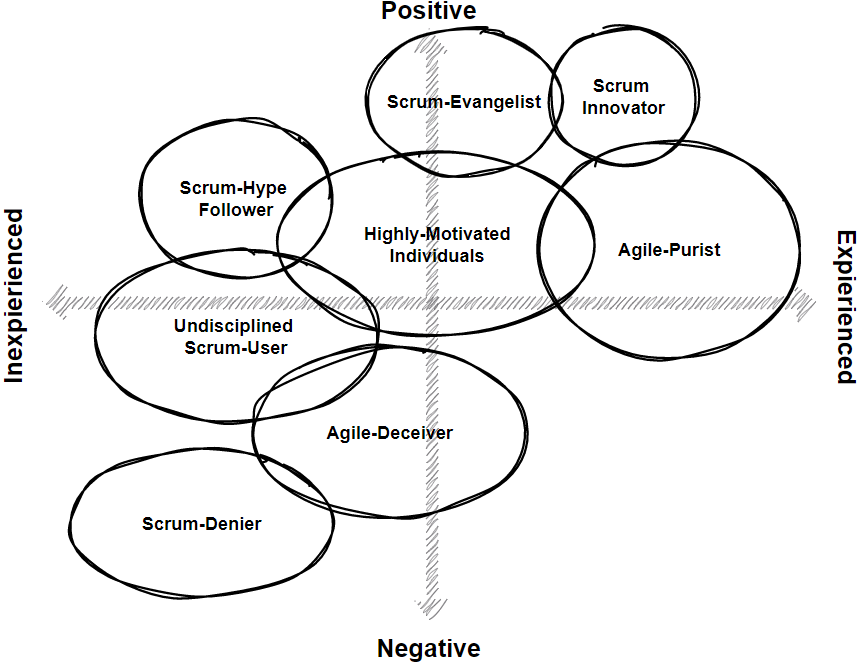
\includegraphics[width=360pt]{./assets/images/opinions-on-scrum.png}}
        \caption{Characters from literature and their views on Scrum}\label{fig:characters-of-agile}
    \end{center}
\end{figure}

% provides a comprehensive understanding
% associated dimension and attribute
\takeaways{
    This section provided a review of previous studies on the theory-practice gap of Scrum, its historical evolution, and its implementation in organizations. Scrum's success has led to the development of various \glspl{framework} based on its \gls{methodology}, including the \ac{safe} and \ac{less}. The latest revisions of the Scrum Guide have emphasized the importance of small teams, clarified the role of the Scrum Master and artifacts, and simplified the language to make it more accessible to a wider audience beyond IT. However, deviations in the roles of Scrum can lead to misunderstandings and frustration, with only one-fourth of organizations following the \glspl{guideline} set forth in the Scrum Guide. In implementing Scrum, reducing command and control structures and changing culture and leadership is important. The ideal situation is where everyone leads themselves, with a flat team model and middle management serving as servant leaders. The client's involvement is crucial for success. Investing in training is recommended to align staff in a common \gls{mindset} and improve product selling. Scaling Scrum's \gls{methodology} in larger organizations requires careful planning and execution to ensure its effectiveness. However, scaling Scrum requires mature individuals, teams, and culture. There are various views and approaches to Scrum, and each has its own impact on the success of the \gls{methodology}. In conclusion, the key takeaway is that the historical evolution of Scrum reflects the growing popularity and continuous efforts to improve its practices and outcomes and that organizations must continuously inspect and adapt their processes to make Scrum effective.
}

\section{Synthesis of findings from previous studies}\label{sec:SynthesisPreviousStudies}
The purpose of this section is to synthesize the findings from previous studies on the theory-practice gap of Scrum. By analyzing the existing body of knowledge, this section aims to provide an overview of common themes and patterns across previous studies. Furthermore, the section will discuss the contributions made by these studies to our overall understanding of the theory-practice gap of Scrum. Finally, the section will identify the gaps in the existing body of knowledge that need further investigation. By doing so, this section will provide a comprehensive overview of the current state of knowledge on the theory-practice gap of Scrum, which will serve as a foundation for future research in this area.

% Summary of common themes and patterns across previous studies
\subsection*{Summary of common themes and patterns}\label{subsec:SummaryOfCommonThemes}
In this analysis, prevalent themes from the existing body of knowledge on the \gls{transformation} or \gls{adaptation} of Scrum in organizations are examined. It has been observed that common misconceptions regarding the roles, \gls{methodology}, and effectiveness of Scrum can result in problematic \glspl{adaptation} due to factors such as lack of training, abstract nature of the \gls{framework}, or inadequate \gls{commitment} to full organizational \gls{transformation}. These issues are rooted in the organizational culture and maturity, as well as the organization's overall goals.

To address these misconceptions, one common solution is to add command and control structures and phase-based sprints rather than goal-oriented sprints. 

Another approach is to reintroduce traditional roles, which often undermines the benefits of flat hierarchical teamwork. Misperceptions about the effectiveness of Scrum at scale are frequently addressed by incorporating control structures and compromising on the \gls{agile} mindset, instead of promoting self-management and iterative product design among \gls{self-managing} teams.

Collaborating with \glspl{client} (when the organization utilizing Scrum is not the \gls{client}) can also pose challenges for organizations early in their \gls{transition}. Attempts to incorporate risk management into the Scrum \gls{methodology} may result in a hit-or-miss development process in phases, rather than involving the domain expert (the \gls{client}) in every increment. It is recommended to train the \gls{client} with internal experts to formulate their ideas for the development teams they engage, rather than predetermining fixed budgets and deadlines.

Failed \glspl{adaptation} or \glspl{transformation} of organizations often stem from a lack of research into which \gls{framework} would best fit the organization's needs. A partial \gls{transformation} that only involves the development team and ignores the rest of the organization may lead to a revert back to traditional \glspl{methodology}. To mitigate this, organizations can seek guidance from external qualified experts who can train management in becoming servant leaders and gradually building trust among former departments.

% Discussion of the contributions of the section to the overall understanding of the theory-practice gap in Scrum 
\subsection*{Discussion of the contribution to the overall undestanding of the theory-practice gap}\label{subsec:DiscussionTheoryPracticeGap}
In this section, the contribution of this thesis to the overall understanding of the theory-practice gap is discussed. The review of existing literature related to the success of Scrum and other \ac{asd} \glspl{framework}, as well as the theory-practice gap, highlights the importance of considering the individual needs of each organization in the implementation process.

The literature suggests that for organizations to realize the full benefits of Scrum, extensive research into their employees' needs, employee training and building trust, ongoing inspection of the Scrum \gls{adoption} status, and collaboration with the \gls{customer} are crucial. However, despite these insights, organizations still face challenges in the \gls{transition} to Scrum, indicating gaps in the current body of knowledge.

\quotethis{If you adopt only one agile practice, let it be retrospectives. Everything else will follow.}{\citeNP{WoodyZuill2014Iya}}

These gaps include the absence of a one-size-fits-all \gls{framework}, a lack of time for researching the organization's needs, limited \gls{commitment} from top management to enforce change, inadequate training in \gls{methodology} and communication, and a need for improvement in the hiring process of external experts.

\newpage

To address these gaps in the body of knowledge, further research is needed to answer the following questions: Why do organizations treat \glspl{framework} as ready-made solutions? Why is there a tendency to rush the process? Why is change management not receiving sufficient support from top management? Why is training in \gls{methodology} and communication not given enough importance? Why are external experts necessary? How can the hiring process of external experts be optimized?

The literature highlights several partial suggestions to address the identified gaps in the implementation of Scrum. According to \citeA[p.~2169]{vanWaardenburg2013Wam}, \ac{asd} serves as a means to identify organizational problems, rather than solving them. 

\citeA[p.~iv]{Rubin2012ESA} emphasizes the importance of listening to the employees' concerns and promoting organizational culture alignment through collaborative decision-making~\cite[p.~234]{Rubin2012ESA}. \citeA[p.~26]{Naseem2009Saa} recommend allocating budget for training early in the \gls{transformation} process. \citeA[pp.~9--13]{Wang2018Taa} advocate for experimenting with the \gls{framework} to gain valuable insights.

Additionally, \citeA[pp.~5--10]{Rubin2012ESA} recommends the use of the Cynefin Framework to determine the suitability of Scrum for an organization. \citeA[p.~101]{Theobald2019Csa} present a model, the Subway Map of Scaling Frameworks, which can assist in comparing different \glspl{framework}.

It is crucial to acknowledge that the failure of a \gls{framework} to meet the needs of an organization does not necessarily indicate a flawed \gls{framework}. However, \citeA[pp.~123--124]{Suryaatmaja2019Tmf} highlight that \glspl{framework} often lack guidance on how to adopt them, which would prove valuable to organizations exploring its use.

\takeaways{
    In this section, the theory-practice gap of Scrum is analyzed. The gap is attributed to common misconceptions about the roles, \gls{methodology}, and effectiveness of Scrum, which stem from the organizational culture, maturity, and goals. The literature stresses the importance of extensive research into employee needs, employee training, building trust, ongoing inspection of the Scrum \gls{adoption} status, and collaboration with the \gls{customer} for organizations to realize the benefits of Scrum. However, organizations still encounter challenges during the \gls{transition} to Scrum, highlighting gaps in the current knowledge base, including the absence of a one-size-fits-all framework, limited \gls{commitment} from top management, inadequate training in \gls{methodology} and communication, and a need for improvement in the hiring process of external experts. Further research is required to address these gaps, including understanding why organizations view \glspl{framework} as ready-made solutions, why change management lacks support, why training in \gls{methodology} and communication is undervalued, and why external experts are necessary. Partial solutions to these gaps include considering the individual needs of each organization, listening to employee concerns, investing in training, experimenting with the framework, and utilizing \glspl{framework} such as Cynefin and Subway Map of Scaling Frameworks.
}